Brugergrænsefladen er opbygget efter designmønstret \gls{MVVM}. \gls{MVVM}-mønsteret adskiller \gls{View}s fra systemets \gls{Model} ved at tilføje en \gls{ViewModel} i mellem de to. Dette gør, at \gls{View}s kan operere uafhængigt af den \gls{Model} som bruges. Det gør også, at dele af \gls{brugergraenseflade}n kan testes nemlig \gls{ViewModel}'en. En overfladisk afbildning af \gls{MVVM}-mønsteret kan ses i figur~\ref{fig:MVVM}\footnote{Billede taget fra: https://en.wikipedia.org/wiki/Model–view–viewmodel}. Da systemet bruger \gls{WPF} og med de førnævte fordele var valget på mønstret faldet på \gls{MVVM}.

\begin{figure}[H]
\centering
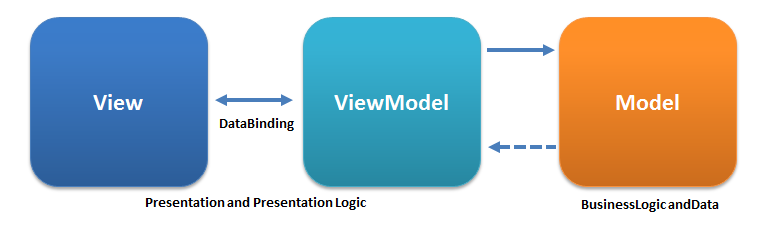
\includegraphics[width=0.8\textwidth]{N+1/MVVMPattern.png}
\caption{MVVM-mønsteret}
\label{fig:MVVM}
\end{figure}

Forbindelsen mellem \gls{View}s og \gls{ViewModel} eksisterer via DataBinding. Dvs. at \gls{View}s kan forbindes via en \textit{property} i vores \gls{ViewModel}. Dette gør det muligt at deklarere et layout i \gls{XAML}, men at holde alt programlogikken i \gls{ViewModel}s.

\logicalview{0.85}{CLASS}{GUI}{pakken GUI}

Når applikationen starter vil der blive oprettet et \texttt{MainWindow}, som har en DataContext, der peger på \texttt{MainViewModel}. Dette illustreres i \ref{fig:GUI_CLASS} med et klassediagram. I \texttt{MainWindow}'s \gls{XAML} kode er de \gls{ViewModel}s, som oprettes i \texttt{MainViewModel}, deklareret. Det gør at de \gls{View}s, som er bundet til de deklarerede \gls{ViewModel}s i \texttt{App.xaml}, vil blive vist i vinduet.

\logicalview{0.85}{CLASS}{Views}{pakken Views i GUI}

På figur~\ref{fig:Views_CLASS} kan bindingerne mellem \gls{View} og \gls{ViewModel} ses. Det vil sige at de bindinger eller \textit{Bindings}, som sker i \gls{XAML} koden binder ned i den pågældende \gls{ViewModel}. Mønsteret gør, at man ikke behøves at have meget \textit{Code Behind}. Ansvaret kan i stedet gives videre til \gls{ViewModel}s.

\logicalview{0.85}{CLASS}{ViewModels}{pakken ViewModels i GUI}

På figur~\ref{fig:ViewModels_CLASS} kan der ses et klassediagram over de \gls{ViewModel}s, som eksisterer i kassesystemet. På figuren er \texttt{MainViewModel} systemets ''Hoved''-\gls{ViewModel}. \texttt{MainViewModel} står for at oprette alle de andre \gls{ViewModel}s og de dertil tilhørende \gls{View}s. Der findes hovedsagligt tre specialiserede \gls{ViewModel}s:
\begin{itemize}
	\item \texttt{SalesViewModel}: Skal håndtere tilføjelse af produkter, betaling og annullere en ordre.
	\item \texttt{TabViewModel}: Skal håndtere produktgrupperne, hvor varene i de valgte gruppe bliver vist, som knapper på brugergrænsefladen.
	\item \texttt{NumpadViewModel}: Skal håndtere de nummererede taster eller det numpad, som findes på brugergrænsefladen.
\end{itemize}

En anden fordel ved at bruge \gls{MVVM} er, at mange af elementerne i \gls{GUI} er dynamisk oprettede. I \texttt{TabView} er alle knapper dynamisk oprettede både ''Tabs'' og ''Product'' knapper. 
Det er \texttt{TabViewModel}, der er ansvarlig for at indhente den data, som skal bruges for at lave \texttt{TabView}. Det eneste der er deklareret i \gls{XAML} for \texttt{TabView} er, hvordan opsætningen skal være.
I forhold til \texttt{SalesView} er den liste af produkter, der er ved at bliver solgt, også lavet dynamisk og opdateres løbende.

\logicalview{0.85}{CLASS}{Dialogs}{pakken Dialogs i GUI}

Dialogerne i \gls{brugergraenseflade}rne bruges, når der er en handling, som kræver brugerens opmærksomhed. Dialogerne kommer f.eks. når der skal vælges en betalingsmetode, eller når kassen skal afstemmes. På Figur~\ref{fig:Dialogs_CLASS} kan følgende klasser ses:
\begin{itemize}
	\item \textbf{PaymentDialog}: Skal håndtere betaling af ordre.
	\item \textbf{BalanceDialog}: Skal håndtere kasse afstemning.
\end{itemize}